\ProvidesFile{chapters/ch-LHC_CMS.tex}

\chapter{THE COMPACT MUON EXPERIMENT AT THE LARGE HADRON COLLIDER}
\label{The_CMS_Experiment_at_the_LHC}

\section{The Large Hadron Collider}
Experiments to discover and determine the properties of SM particles are performed at particle accelerator facilities.
The Large Hadron Collider (LHC) is a $\SI{27}{\km}$ circular particle accelerator located at the European Center for Nuclear Research (CERN) designed to accelerate two counter-rotating proton beams to energies up to $\SI{6.8}{\TeV}$ ($99.999999\%$ the speed of light) and collide them at designated interaction points (IP).
The LHC is the largest and most powerful particle accelerator ever built; its design, construction, and operation are towering engineering achievements of mankind, requiring an international collaboration of thousands of scientists, engineers, and technicians from more than 100 countries.
The successful operation of the LHC has contributed to our understanding of the fundamental nature of matter by providing conditions to test the hypotheses of the SM and enabling many important discoveries in particle physics.
The primary design criteria for the LHC was to provide conditions for elucidating the nature of EWSB, testing the hypothesis of the BEH mechanism, and discovering the Higgs boson.

\subsection{Probing Small Scales with High Energy}
The De Broglie relation states that the wavelength of a particle is inversely proportional to its energy.
According to Heisenberg's uncertainty principle, the position of a particle with a short wavelength cannot be precisely determined.
Thus, the motivation for building higher energy particle colliders is to probe smaller distance scales.
In the 20th century, particle accelerator energy increased many orders of magnitude from \sim$\SI{100}{\keV}$ in the 1930s to \sim$\SI{10}{\TeV}$ in the 2010s (see table~\ref{energy_distanceprobed}), and current distance scales probed are down to \sim$\SI{e-19}{\m}$.
\begin{table}[!htb]
\begin{center}
\begin{math}
\begin{array}{|c|c|c|}
\hline \text { Decade } & \text { Energy } & \text { Distance Probed } \\
\hline 1930 & \sim \SI{100}{\keV} & \sim \SI{e-11}{\m} \\
\hline 1950 & \sim \SI{100}{\MeV} & \sim \SI{e-14}{\m} \\
\hline 1970 & \sim \SI{100}{\GeV} & \sim \SI{e-17}{\m} \\
\hline 1990 & \sim \SI{1}{\TeV} & \sim \SI{e-18}{\m} \\
\hline 2010 & \sim \SI{10}{\TeV} & \sim \SI{e-19}{\m} \\
\hline
\end{array}
\end{math}
\caption{In the 20th century, particle accelerator energy increased many orders of magnitude from \sim$\SI{100}{\keV}$ in the 1930s to \sim$\SI{10}{\TeV}$ in the 2010s, and current distance scales probed are down to \sim$\SI{e-19}{\m}$.
        }
\label{energy_distanceprobed}
\end{center}
\end{table}

\subsection{Accelerator Complex at CERN}
Before reaching the LHC, protons must first be accelerated through a series of smaller accelerators at CERN's accelerator complex.
A schematic of the LHC at CERN's accelerator complex in Geneva at the border of Switzerland and France is shown in figure~\ref{CERN_LHC}.
\begin{figure}[!htb]
  \begin{center}
    \begin{tabular}{c}
        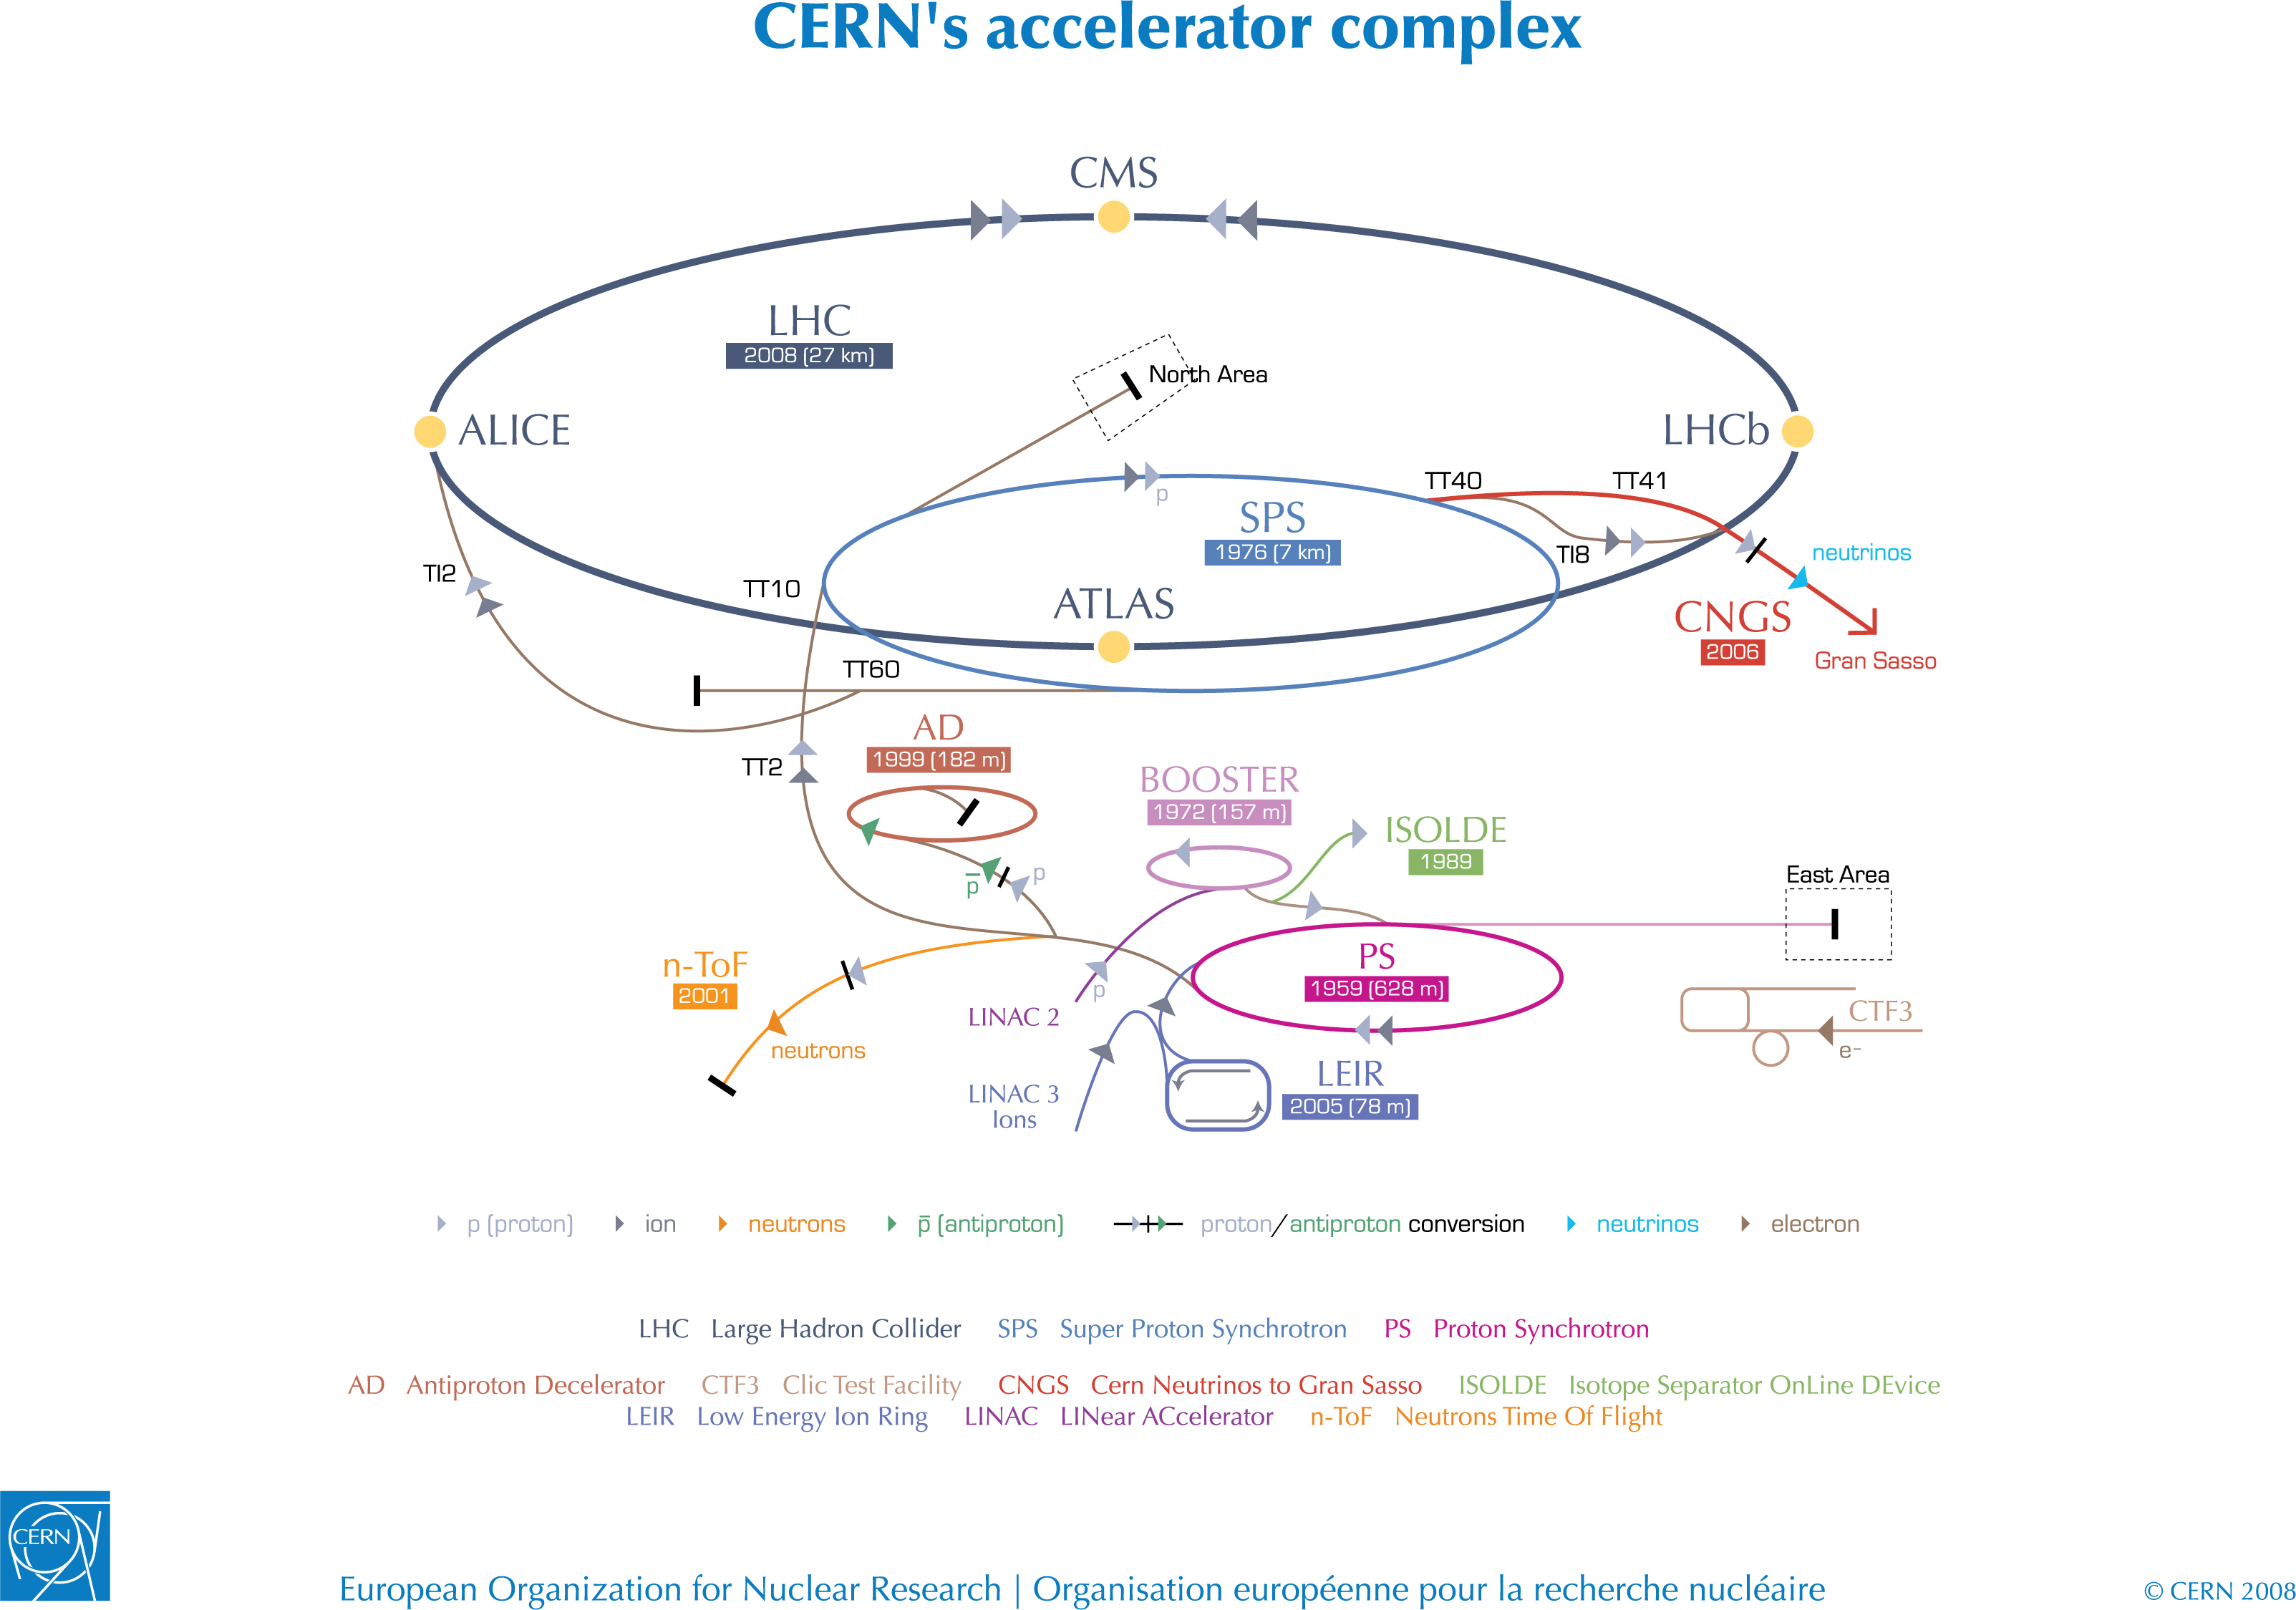
\includegraphics[width=0.9\textwidth]{fig_LHC_CMS/CERN_LHC.png}
    \end{tabular}
    \caption{A schematic of the LHC at CERN's accelerator complex in Geneva at the border of Switzerland and France~\cite{Christiane:1260465}.
            }
    \label{CERN_LHC}
  \end{center}
\end{figure}
Protons are produced from hydrogen gas by inducing electric discharge in a duoplasmatron.
The $\SI{80}{\m}$ Linear Accelerator 2 (Linac 2) accelerates protons to an energy of $\SI{160}{\MeV}$ before injecting them into the $\SI{157}{\m}$ circumference Proton Synchrotron Booster (PSB), which divides the beam into bunches consisting of more than 100 billion protons with $\SI{25}{\ns}$ separation, and further increases the proton energy to $\SI{2}{\GeV}$.
Next, the proton bunches are injected into the $\SI{628}{\m}$ circumference Proton Synchrotron (PS), which accelerates the bunches to $\SI{26}{\GeV}$ before injecting them into the $\SI{7}{\km}$ circumference Super Proton Synchrotron (SPS), which increases the proton energy to $\SI{450}{\GeV}$ before finally injecting them into the LHC, which accelerates them to their final (2016, 2017, and 2018) energy of $\SI{6.5}{\TeV}$.

Ultra-high vacuum conditions \sim$\SI{e-11}{\mbar}$ are maintained in the LHC beam pipes and 16 radiofrequency (RF) cavities with electric fields oscillating at a frequency resonant with the bunching frequency are used to accelerate the protons.
Superconducting magnetic cooled with superfluid helium to temperatures below $\SI{2}{\K}$ and operating at fields exceeding $\SI{8}{\T}$~\cite{LyndonEvans_2008} are used to shape and control the beam directions.
1232 dipole magnets bend the beams around the ring and 474 quadrupole magnets are used to focus and collimate the beams.
The $\SI{25}{\ns}$ bunch separation corresponds to 2808 proton bunches simultaneously in the LHC.
At the four LHC IPs, proton bunches cross at a rate of $\SI{40}{\MHz}$, creating collisions corresponding to temperatures a billion times hotter than the core of the sun.
Final states after the collisions are measured and recorded by the CMS, ATLAS, ALICE, and LHCb particle detectors.

\subsection{Luminosity}
When two particle beams cross paths in a particle accelerator, the number of events of a particular process that occur per second is given by:
\begin{linenomath*}
\begin{align}
{\frac{dN_{\text {Events}}}{dt}}= \mathcal{L}_{\text{Inst}} \cdot \sigma_{\text{Process}}
\end{align}
\end{linenomath*}
where $\mathcal{L}_{inst}$ is the instantaneous luminosity and $\sigma_{\text{Process}}$ is the cross-section of the process under consideration.
For the \beamenergy LHC, the total cross-section for all inelastic processes has been measured to be $\sigma_{\text{Inelastic}} = 68.6 \pm 0.5 \; (\text{Syst}) \; \pm 1.6 \; (\text{Lumi}) \; \si{\milli \b}$~\cite{inelasticprotonprotoncrosssection}.
The instantaneous luminosity can be parameterized~\cite{Karacheban:2294183} as:
\begin{linenomath*}
\begin{align}
\mathcal{L}_{\text{Inst}}=\frac{N_b^2 n_b f_{\mathrm{rev}}}{A_{eff}}
\end{align}
\end{linenomath*}
where $N_b = \num{1.15e11}$ is the number of particles per bunch, $n_b=2808$ the number of bunches per beam, $f_{\mathrm{rev}} = \SI{11245}{\Hz}$ the revolution frequency in the collider, and $A_{eff} = \sqrt{\varepsilon_x \beta_x \varepsilon_y \beta_y}$ is the effective area of the luminous region, where $\beta_{x,y}$ and $\varepsilon_{x,y}$ are the beam amplitude and emittance transverse to the beam axis, and is measured regularly during Van der Meer (VdM) scans.
$\mathcal{L}_{\text{Inst}}$ decays over time due to the intensity degradation and beam emittance, with a mean life of \sim$\SI{15}{\h}$~\cite{LyndonEvans_2008}.
The high $\mathcal{L}_{\text{Inst}}$ of the LHC typically results in many proton-proton interactions per bunch crossing.
The number of collisions per bunch cross is referred to as pile-up (PU), and is quantified as:
\begin{linenomath*}
\begin{align}
PU = \frac{\mathcal{L}_{\text{Inst}} \cdot \sigma_{\text{Inelastic}}}{n_b f_{\mathrm{rev}}}
\end{align}
\end{linenomath*}
Typical PU in CMS recorded data from 2016 through 2018 was around 20-30 interaction vertices per bunch crossing, but high (low) extremes routinely occurred during the beginning (end) of beam fills due to instantaneous 
luminosity decay.
For a particular process, the total number of events that occur in a recorded data set is given by:
\begin{linenomath*}
\begin{align}
N_{\text {Events}}= \mathcal{L} \cdot \sigma_{\text{Process}}
\end{align}
\end{linenomath*}
where $\mathcal{L} = \int \mathcal{L}_{\text{Inst}} \,dt$ is the instantaneous luminosity integrated over the corresponding period of time the data was recorded, i.e. the integrated luminosity.

\subsection{Upcoming High Luminosity - LHC Phase}
During 2016, 2017, and 2018, the LHC operated with beam energies of $\SI{6.5}{\TeV}$, corresponding to center-of-mass collision energies of $\SI{13}{\TeV}$.
Recently, the LHC finished upgrading the beam energies to $\SI{6.8}{\TeV}$.
After operating at $\sqrt{s}=\SI{13.6}{\TeV}$ through 2025, the LHC plans to vastly increase the instantaneous luminosity, and substantial R\&D effort is being done now to prepare accelerator and detector upgrades for high luminosity (HL-LHC) environments.

\section{The Compact Muon Solenoid Detector}
Particle detectors measure electrical signals and collect scintillated light produced by particles interacting with the material of the detector.
The Compact Muon Solenoid (CMS) is a general-purpose detector, built for testing predictions of the SM, exploring models BSM, and discovering NP.
The primary design benchmarks for CMS were precision studies of QCD, electroweak, and flavor physics, as well as detection of the Higgs boson.
CMS is a collection of sub-detectors that are layered cylindrically around the IP, with barrel and end-cap/disk components, that provide the detector with near-hermetic coverage of the solid angle.
An exploded view of the CMS detector layout with labeled sub-detectors is shown in figure~\ref{CMS_Detector}.
\begin{figure}[!htb]
  \begin{center}
    \begin{tabular}{c}
        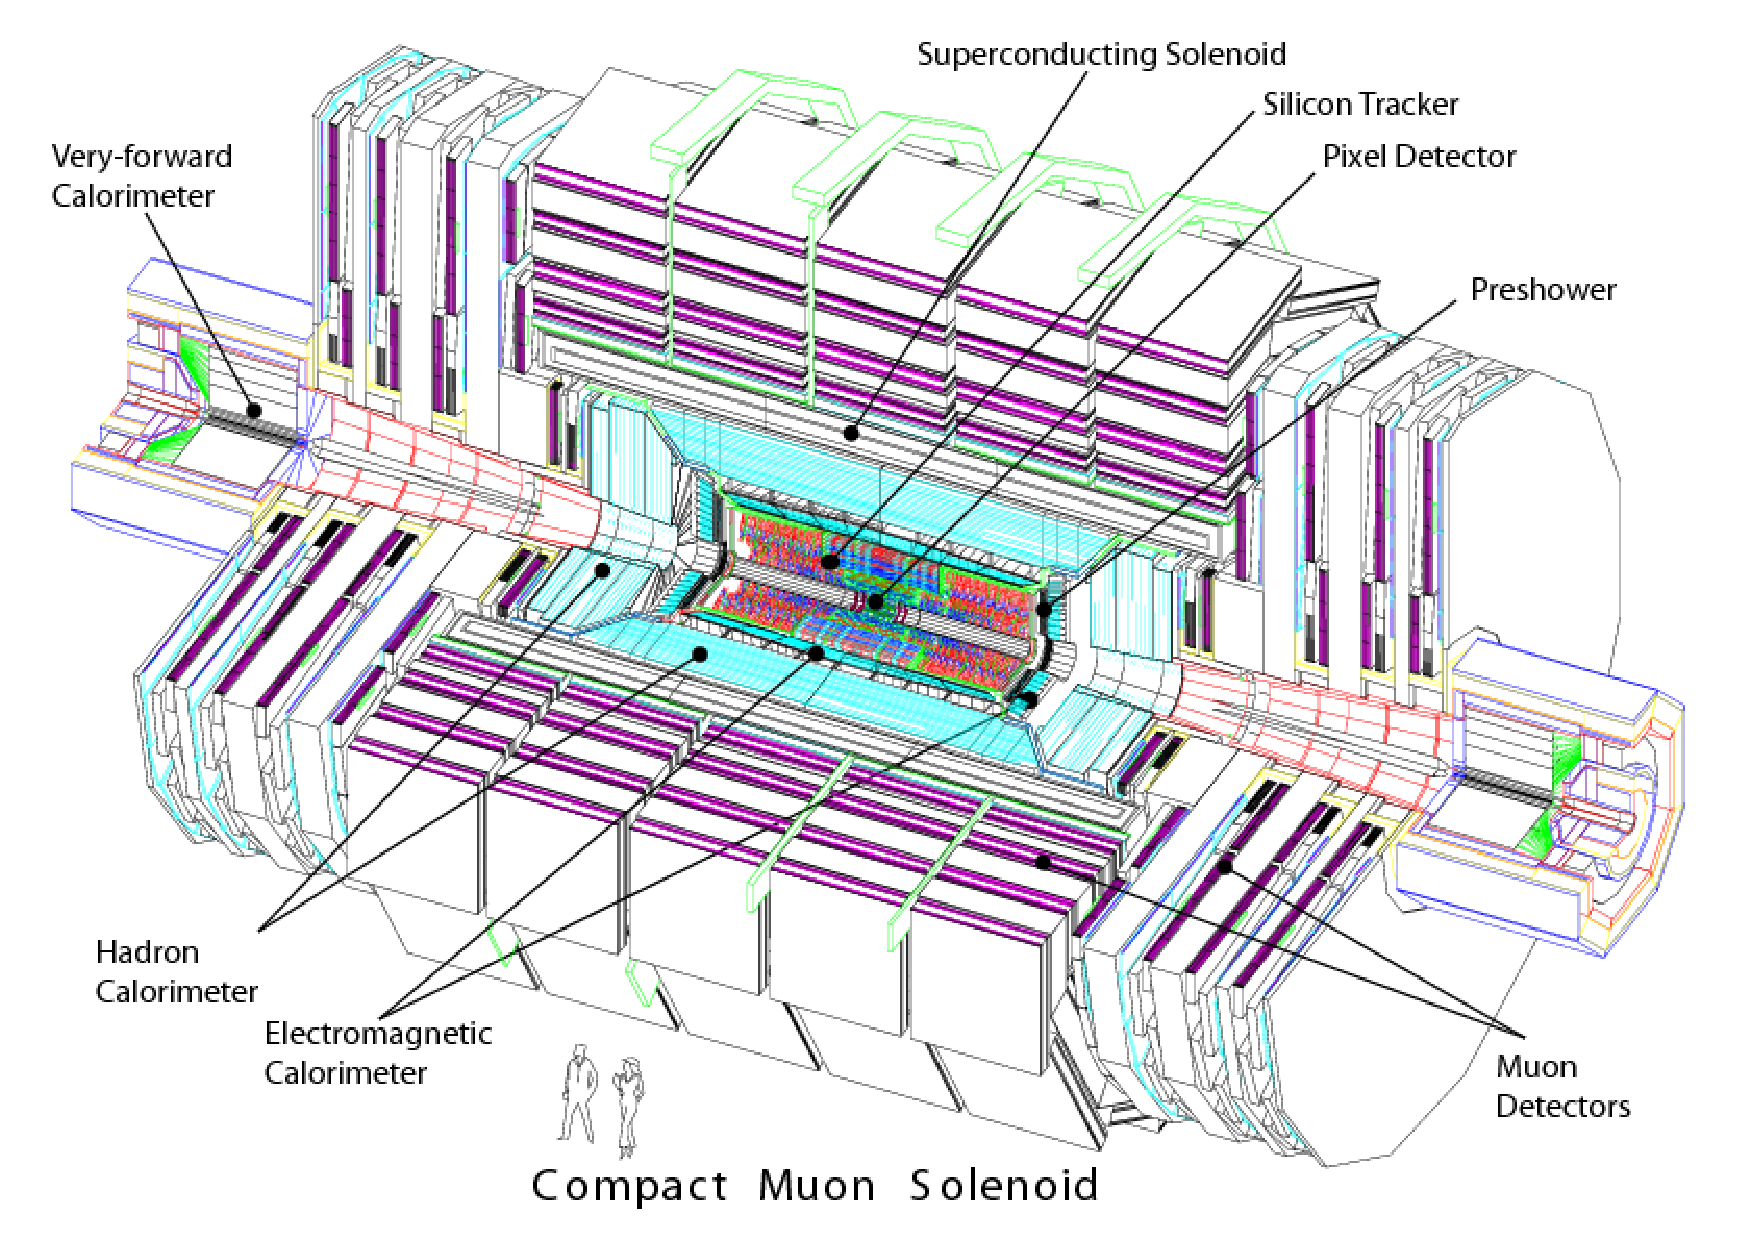
\includegraphics[width=0.9\textwidth]{fig_LHC_CMS/CMS_Detector.pdf}
    \end{tabular}
    \caption{An exploded view of the CMS detector layout with labeled sub-detectors~\cite{Bayatian:922757}.
            The human figures are included for scale.
            }
    \label{CMS_Detector}
  \end{center}
\end{figure}
Overall, the CMS detector is $\SI{21.6}{\m}$ long, with a diameter of $\SI{14.6}{\m}$, and weighs more than $\SI{12500}{\t}$.

\subsection{Coordinate System}
\label{CMS_Coordinate_System}
The CMS origin is located at the nominal interaction point of the beams at the center of the experiment.
The $\hat{y}$-axis points vertically upward, the $\hat{z}$-axis is along the beam line, and the $\hat{x}$-axis points towards the center of the LHC ring.
When analyzing the kinematics of high-energy particle collisions, it is more conventional to use the $\pT$, $\eta$, $\phi$ coordinate system:
\begin{itemize}
\item The transverse momentum $\pT = \sqrt {{p_x}^2+{p_y}^2}$ is the momentum component of a particle perpendicular to the beam axis. 
\item The pseudorapidity $\eta$ is a measure of the angle between the particle's momentum vector and the beam axis.
Pseudorapidity is defined as: 
\begin{linenomath*}
\begin{align}
\eta=\frac{1}{2} \ln \frac{\vert\vec{p}\vert+p_z}{\vert\vec{p}\vert-p_z}=-\ln \left[\tan \left(\frac{\theta}{2}\right)\right]
\end{align}
\end{linenomath*}
in terms of the polar angle $\theta$, which is measured from the z-axis.
For particles with $m {{\ll}\!\!\!\!/} \; \vert \vec{p} \vert$, it is sometimes preferable to use rapidity, defined as:
\begin{linenomath*}
\begin{align}
y=\frac{1}{2} \ln \frac{E+p_z}{E-p_z}
\label{Rapidity}
\end{align}
\end{linenomath*}
which converges to pseudorapidity in the ultra-relativistic limit.
One advantage of using pseudorapidity (rapidity) is that differences in $\eta$ ($y$) are Lorentz invariant for longitudinal Lorentz boosts along the beam axis.
\item The azimuthal angle $\phi$ is the angle in the transverse plane between the particle's momentum vector and the $\hat{x}$-axis.
\end{itemize}
The energy $E$ of a particle, together with its 3-vector $\langle \pT, \eta, \phi \rangle$, form a 4-vector $(E,\pT, \eta, \phi)$ that fully characterizes the particle's momentum and energy in space and time.

A measure of angular separation between objects $i$ and $j$ can be defined using $\eta$ and $\phi$ coordinates:
\begin{linenomath*}
\begin{align}
\Delta R_{ij} = \sqrt {{(\phi_i - \phi_j)}^2+{(\eta_i - \eta_j)}^2};
\label{DeltaR}
\end{align}
\end{linenomath*}
this quantity is useful for clustering particle showers into jets and rejecting events with overlapping objects.

\subsection{Solenoid Magnet}
Central to the design of the CMS detector, and the source of its name, is the $\SI{12.9}{\m}$-long, $\SI{5.9}{\m}$ inner diameter, $\SI{200}{\t}$, niobium-titanium alloy superconducting solenoid, providing an axial and uniform $\SI{3.8}{\T}$ magnetic field within the solenoid, and a return field outside the solenoid that is confined by an iron yoke that contains and guides the field.
The solenoid is large enough that the inner tracking detectors and calorimeters fit inside, which advantageously eliminates energy losses caused by showering in the coil material before energy can be measured in the calorimeters.
The magnetic field of the solenoid, depicted in figure~\ref{Solenoid}, bends the paths of charged particles as they move through the detector, enabling the tracker to make good resolution measurements of their transverse momentum and charge from their curvature.
\begin{figure}[!htb]
  \begin{center}
    \begin{tabular}{c}
        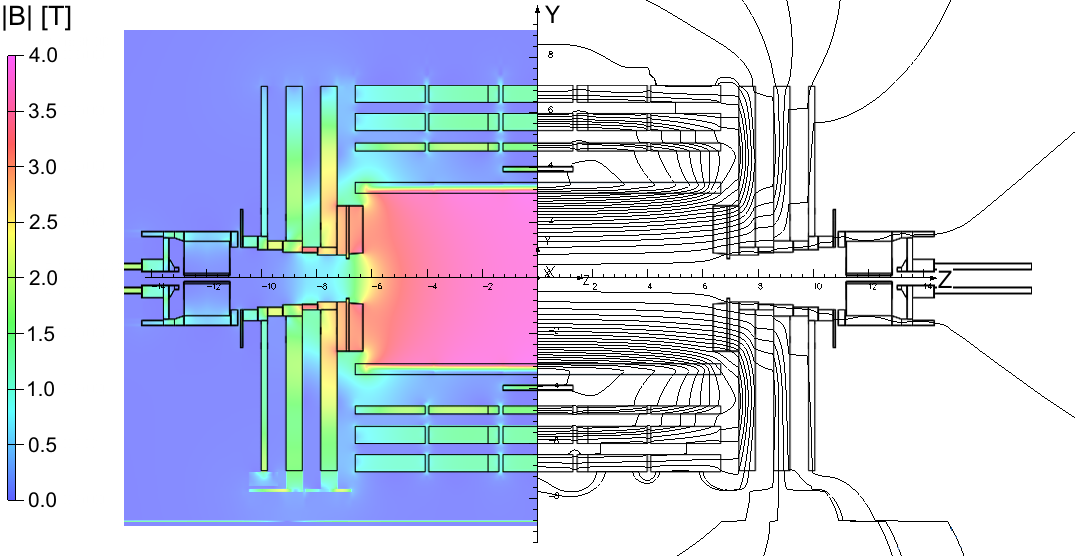
\includegraphics[width=0.65\textwidth]{fig_LHC_CMS/Solenoid.png}
    \end{tabular}
    \caption{Magnitude of magnetic field (Left) and field lines (Right) simulated on a longitudinal section of the CMS detector~\cite{Chatrchyan:1215500}.
            }
    \label{Solenoid}
  \end{center}
\end{figure}


\subsection{Silicon Inner Tracker}
The inner tracker consists of silicon pixel detectors surrounded by silicon strip detectors.
Silicon detector technology provides high granularity, fast response, radiation hardness, and efficient cooling, while also minimizing material to limit multiple scattering, bremsstrahlung, photon conversion and nuclear interactions.
High-energy charged particles ionize the silicon as they traverse the detectors, leaving trails of position measurements which are used to reconstruct the particle trajectories with sophisticated algorithms.
The magnetic field of the solenoid exerts a force perpendicular to a charged particle transverse momentum, and transverse momentum magnitude is measured from the curvature of its trajectory.
The inner tracker cylindrical volume of length $\SI{5.8}{\m}$ and diameter $\SI{2.6}{\m}$ covers out to $\vert \eta \vert < 2.5$ and is separated into the barrel and forward regions.

The silicon pixel tracker operates closest to the IP, in the region with the highest radiation and particle flux from the $pp$ collisions.
The primary limiting factor for impact parameter resolution is the radial distance of the innermost tracking layer.
In the barrel region, three layers of pixel detectors, $\SI{53}{\cm}$ long, are at radial distances $r = 4.4, 7.3, 10.2 \si{\cm}$ from the beam, while in the forward regions, two end-cap disks with radii $\SI{6}{\cm}$ and $\SI{15}{\cm}$ are placed on each side at $z = \pm \SI{34.5}{\cm}$ and $\SI{46.5}{\cm}$.
The doping scheme for the pixels is $n$-on-$n$, which can be operated partially depleted even at high fluence.
To minimize occupancy in the inner region of high particle flux and achieve good vertex resolution for the identification primary and secondary vertices, pixel detectors are high granular and finely segmented in two dimensions with pixel size $\approx 100 \times 150 \; \mu \si{\m \squared}$.
The pixel detector consists of 1440 modules that cover a total area of $\approx \SI{1}{\m \squared}$, so altogether it contains about 66 million pixels.
In the barrel region, $r-\phi$ resolution is improved through charge-sharing among pixels due to the Lorentz effect, while in the forward region, modules are rotated in a turbine-like geometry to improve the resolution by inducing charge-sharing.
The spatial resolution of the pixel detector is $10 \; \mu \si{\m}$ ($20 \; \mu \si{\m}$) for $r-\phi$ ($z$) measurements.

During the LHC winter shutdown between 2016 and 2017, the entire pixel tracker was replaced (see figure~\ref{Inner_Tracker}) with the Phase-1 upgrade~\cite{Lipinski_2017}.
A fourth layer was added in the barrel region , the radius of the innermost layer was reduced from $r = \SI{4.4}{\cm}$ to $r = \SI{2.9}{\cm}$, a fifth layer was added in the forward regions, and the total number of pixels increased to 124 million.
The cooling system was replaced with evaporative \ce{CO2} cooling technology, which efficiently removes heat using of the latent heat of vaporization.
After the replacement, the silicon inner tracker altogether contributes total radiation length up to \sim$0.5 X_0$ and total interaction length up to \sim$1.8 \lambda_I$, mostly from supports, cables, and cooling~\cite{Sirunyan:2270046}.
\begin{figure}[!htb]
  \begin{center}
    \begin{tabular}{cc}
        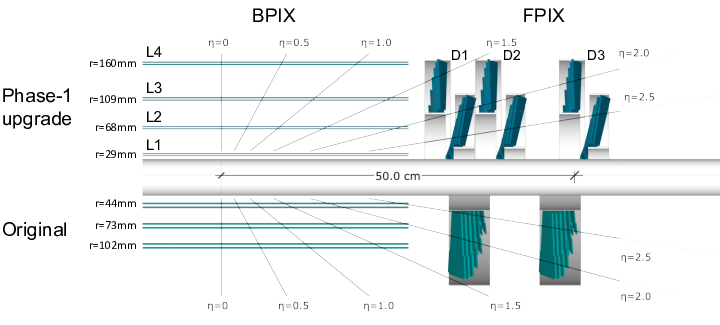
\includegraphics[width=0.45\textwidth]{fig_LHC_CMS/Pixel_Upgrade.png}
        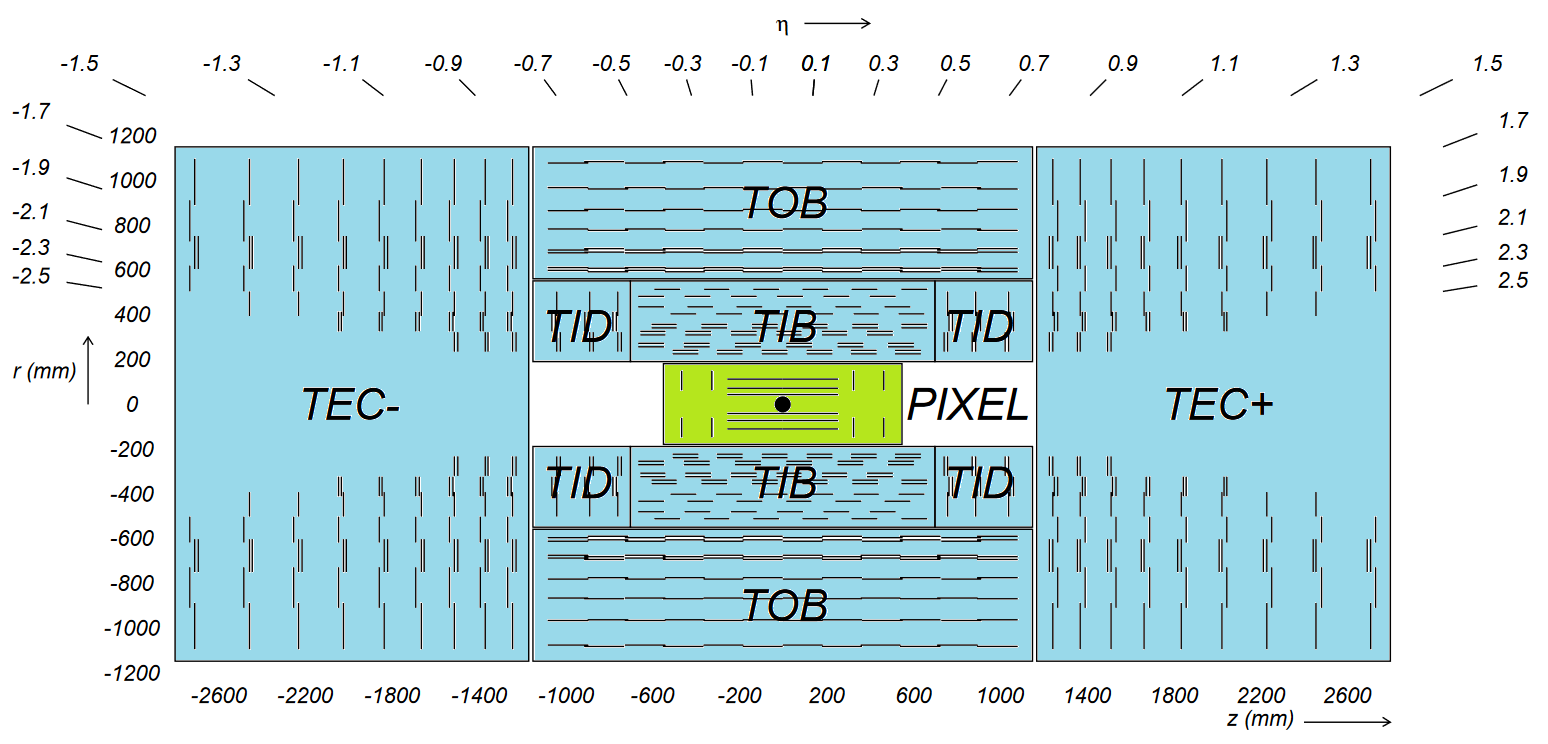
\includegraphics[width=0.45\textwidth]{fig_LHC_CMS/Inner_Tracker.png}
    \end{tabular}
    \caption{Silicon Pixel Tracker (Left) before and after the Phase-1 upgrade~\cite{Adam_2021}.
             Silicon Inner Tracker before Pixel Phase-1 upgrade (Right): ~\cite{Chatrchyan:1211825}.
            }
    \label{Inner_Tracker}
  \end{center}
\end{figure}

Surrounding the pixel tracker is the silicon strip tracker (see figure~\ref{Inner_Tracker}), consisting of 15,148 modules with 24,244 silicon sensors, that cover a total area of $\approx \SI{198}{\m \squared}$, and altogether contains 9.6 million microstrips.
In the barrel region, the strip tracker is separated into the Tracker Inner Barrel (TIB), which covers from $\SI{20}{\cm} < r < \SI{55}{\cm}$ out to $z = \pm \SI{65}{\cm}$, and the Tracker Outer Barrel (TOB), which covers from $\SI{55}{\cm} < r < \SI{116}{\cm}$ out to $z = \pm \SI{118}{\cm}$.
In the forward regions, the strip tracker is separated into the Tracker Inner Disks (TID$^\pm$), which cover $\pm\SI{65}{\cm} < z < \pm\SI{124}{\cm}$ and $\SI{20}{\cm} < r < \SI{55}{\cm}$, and Tracker End-Caps (TEC$^\pm$), cover $\pm\SI{124}{\cm} < z < \pm\SI{282}{\cm}$ and $\SI{22.5}{\cm} < r < \SI{113.5}{\cm}$.
The doping scheme for strips is $p$-on-$n$, which undergoes type inversion after enough radiation damage to the crystal lattice and change.
Strips are only finely segmented in one dimension, with minimum cell sizes of  $\approx \SI{10}{\cm} \times 80 \; \mu \si{\m}$ in the TIB and TID, and maximum cell sizes of $\approx \SI{25}{\cm} \times 180 \; \mu \si{\m}$ in the TOB and TEC.
The TIB (TOB) has four (six) layers of silicon microstrip detectors, providing up to four (six) $r-\phi$ measurements, while the TID (TEC) has four (nine) layers, providing up to four (nine) $z-\phi$ measurements.
The single point resolutions of these measurements are $23-35 \; \mu \si{\m}$ in the TIB, $23-35 \; \mu \si{\m}$ in the TOB.
Some layers additionally have modules mounted with stereo angles to provide measurements of the second coordinate ($z$ in the barrel region and $r$ in the forward regions).
The single point resolutions of these measurements are $\approx 230 \; \mu \si{\m}$ in the TIB, $\approx 530 \; \mu \si{\m}$ in the TOB.
The hit efficiency of the silicon strip tracker is 99.8\%.

\subsection{Electromagnetic Calorimeter}
Surrounding the silicon inner tracker is the electromagnetic calorimeter (ECAL), consisting of 61,200 lead tungstate (\ce{PbWO4}) scintillating crystals in the barrel region (EB) and 7,324 crystals in each of the end-caps (EC).
The EB covers out to $\vert \eta \vert < 1.479$, with inner radius $\SI{1.29}{\m}$, while the EE covers $1.479 < \vert \eta \vert < 3.0$, at a longitudinal distance $\vert z \vert = \SI{3.15}{\m}$ from the IP (see figure~\ref{ECAL_HCAL}).

The ECAL measures the energy of particles, such as electrons, positrons, and photons, that primarily interact through the electromagnetic force.
Lead tungstate is high density $\SI{8.28}{\g\per\cm\cubed}$, optically transparent, radiation-hard, fast, and has a short radiation length ($X_0 = \SI{0.89}{\cm}$).
The crystals have a highly-granular $22 \times 22 \si{\mm\squared}$ ($28.6 \times 28.6 \si{\mm\squared}$) front-face cross-section in the EB (EE) that matches the Molière radius of lead tungstate, i.e. the radius of a cylinder that contains a fraction $90 \%$ of the energy deposited by the shower.
The crystal lengths are $\SI{23}{\cm}$ ($\SI{22}{\cm}$) in the EB (EE), corresponding to a total radiation length of $25.8X_0$ ($24.7X_0$).
The total radiation length of the crystals essentially guarantees that electrons and photons will deposit all of their energy in the ECAL, resulting in an electromagnetic shower that excites nearby atoms which subsequently relax by scintillating light.
The scintillation decay time of lead tungstate is less than $\SI{25}{\ns}$, and it scintillates a blue-green light.
The crystals are fully polished to totally internally reflect light down the crystal where it is collected by a silicon avalanche photodiodes in the EB and vacuum phototriodes in the EE, which are designed to be radiation-hard operate in the high magnetic field.
In the $1.653 < \vert \eta \vert < 2.6$ region are preshower detectors that are primarily designed to distinguish photons originating from $\pi^0$ decays.

\begin{figure}[!htb]
  \begin{center}
    \begin{tabular}{cc}
        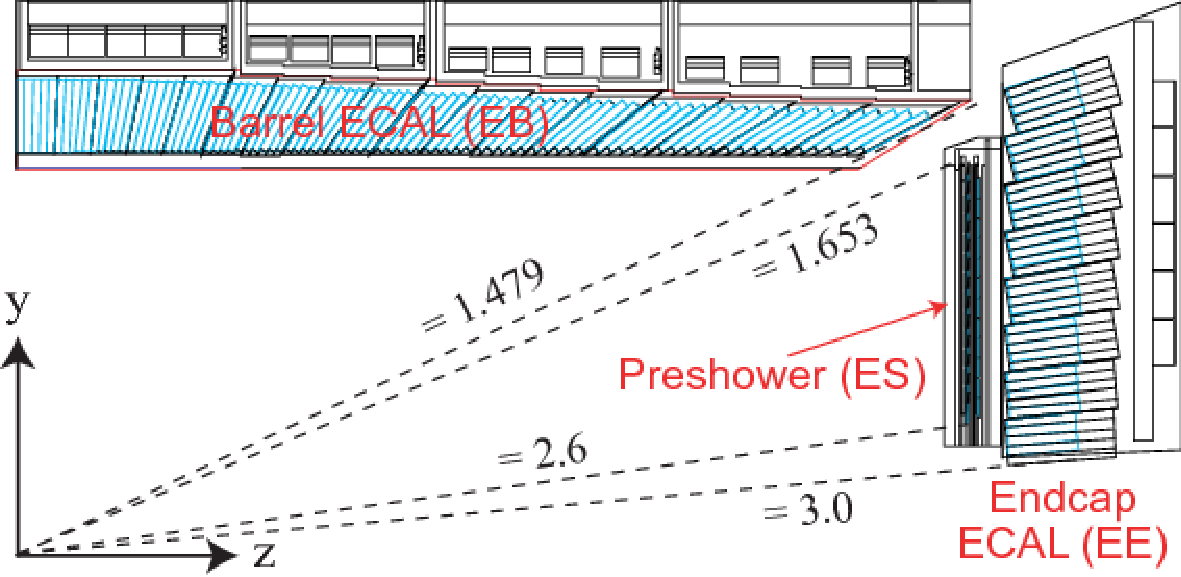
\includegraphics[width=0.45\textwidth]{fig_LHC_CMS/ECAL.pdf}
        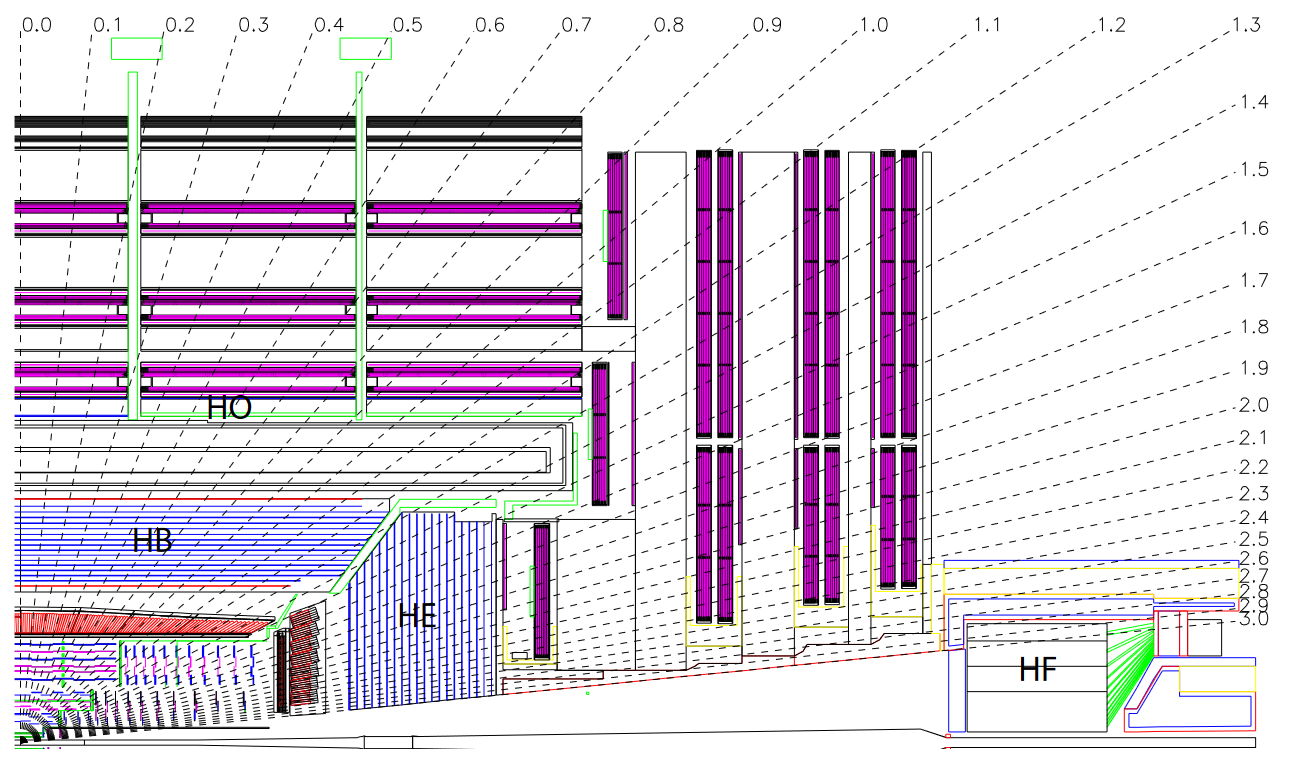
\includegraphics[width=0.40\textwidth]{fig_LHC_CMS/HCAL.png}
    \end{tabular}
    \caption{Schematic views of the ECAL (Left) ~\cite{Bayatian:922757} and HCAL (Right) ~\cite{Chatrchyan:1129810}.
            }
    \label{ECAL_HCAL}
  \end{center}
\end{figure}

\subsection{Hadronic Calorimeter}
Outside the ECAL is the hadronic calorimeter (HCAL), consisting of the HCAL Barrel (HB), which covers out to $\vert \eta \vert < 1.3$, the HCAL End-caps (HE), which cover $1.3 < \vert \eta \vert < 3$, and radiation-hard, quartz fibre hadron calorimeters that are placed in the forward region (HF) $3 < \vert \eta \vert < 5.2$ (see figure~\ref{ECAL_HCAL}).
The HCAL is designed to measure jet energy by forcing their strongly-interacting hadron constituents to shower in brass absorber layers that alternate with scintillating plastic layers, in which the showers deposit their energy by exciting nearby atoms which subsequently relax by emitting light collected by hybrid photodiodes.
The non-magnetic brass absorber layer is composed of 70\% \ce{Cu} and 30\% \ce{Zn}, has a nuclear interaction length of $\lambda_I = \SI{16.42}{\cm}$.
In the barrel region, the HB does not have sufficient total interaction length for hadron showers to completely exhaust their energy in the calorimeter, so an Outer HCAL (HO) of scintillating plastic layers, that uses the solenoid as an additional absorber layer, is placed outside the solenoid and covers out to $\vert \eta \vert < 1.3$.
The ECAL, which radially precedes the HCAL, contributes $1.1\lambda_I$.
At $\eta = 0$, the total interaction length of the absorber layers is $5.82\lambda_I$, and increases with $\eta$, so that at $\vert \eta \vert = 1.3$ it is $10.6\lambda_I$.

\subsection{Muon Outer Tracker}
Unlike most particles, muons are not stopped by any of the calorimeters, superconducting solenoid, or iron flux-return yoke. 
Four layers of chambers to detect muons are placed at the very outer layers of the experiment in the iron flux-return yoke. 
The muon system is designed with three different types of gaseous particle detectors: 
\begin{itemize}
\item drift tube (DT) chambers covering $\vert \eta \vert < 1.2$,
\item cathode strip chambers (CSC) covering $0.9 < \vert \eta \vert < 2.4$, and
\item resistive plate chambers (RPC) covering $\vert \eta \vert < 1.6$.
\end{itemize}
The layout for one quadrant of the muon system is shown in figure~\ref{Muon_System}.
The RPCs have inferior spatial resolution compared to the DTs and CSCs, but have excellent timing resolution and are primarily used for muon triggering.
The muon system is aligned with the inner tracker in order for the detectors to work together to identify muons and reconstruct their trajectories.
\begin{figure}[!htb]
  \begin{center}
    \begin{tabular}{c}
        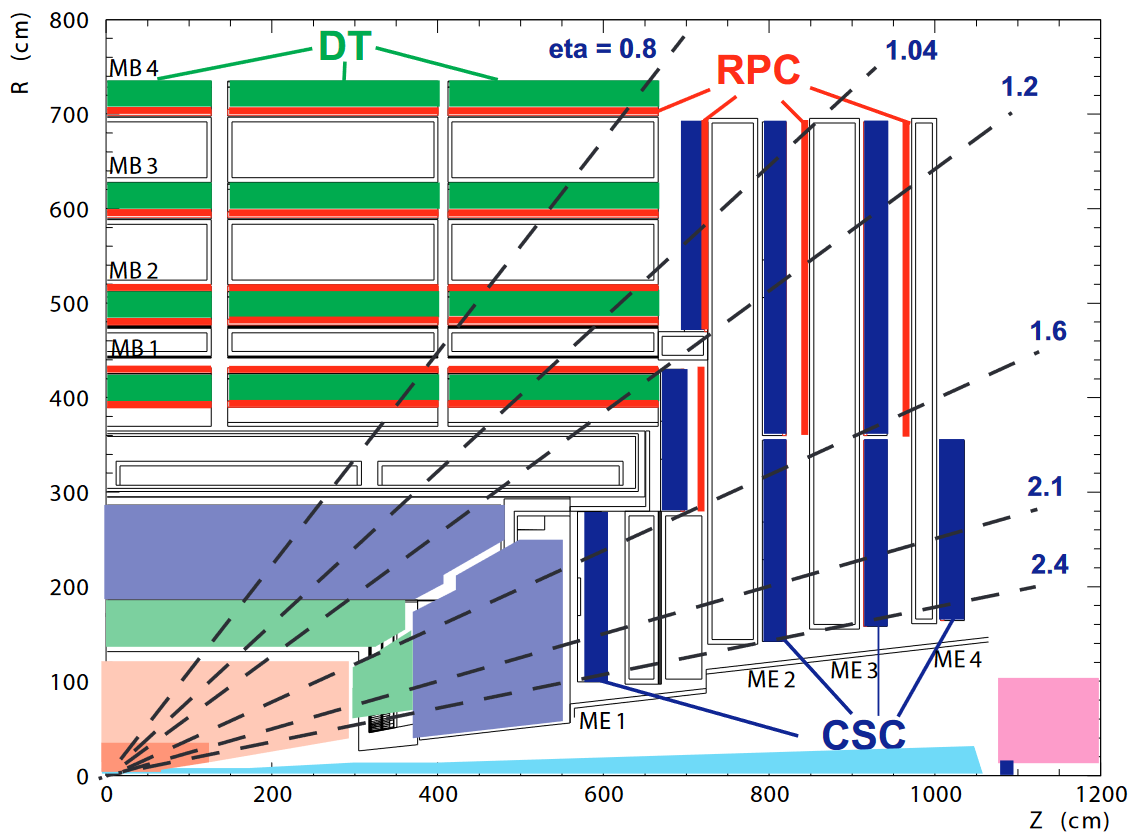
\includegraphics[width=0.65\textwidth]{fig_LHC_CMS/Muon_System.png}
    \end{tabular}
    \caption{Layout of one quarter of the CMS muon system~\cite{Bayatian:922757}.
            }
    \label{Muon_System}
  \end{center}
\end{figure}

\subsection{Trigger and Data Acquisition System}
CMS wants to collect the most relevant data from bunch crossings with a $\SI{40}{\MHz}$ event rate.
Each bunch crossing generates \sim$\SI{1}{\M \byte}$ of data, but due to limited bandwidth, the detectors cannot readout and store \sim$\SI{40}{\T \byte \per \s}$, so a trigger system is necessary to reject the least interesting 99.9999\% of events in quasi-real time, and reduce the event rate to \sim$\SI{1}{\kilo \Hz}$ before storage.
This is not an unreasonable constraint, as the total cross-section of proton-proton interactions (elastic and inelastic) at \beamenergy is \sim$\SI{100}{\milli \b}$, while interesting processes such as top quark pair production and Higgs boson production have cross-sections on the orders of \sim$\SI{800}{\pico \b}$ and \sim$\SI{50}{\pico \b}$ respectively.
To accomplish this, CMS has a highly reliable and efficient trigger system, composed of detector electronics, a level-1 (L1) hardware trigger, a readout network, and a high level software trigger (HLT).
The L1 trigger uses hardware processors and raw readouts from the calorimeters and muon systems to reduce the event rate to \sim$\SI{100}{\kHz}$ with a latency of $3.8 \; \mu s$.
The data acquisition then passes the complete readout of the event data to the HLT, which has a latency of $320 \; \mu s$ perform fast reconstruction and event selection to filter events and reduce the rate of stored events to \sim$\SI{1}{\kilo \Hz}$.
The events that pass the HLT filter are saved for offline analysis to one or several HLT paths, which correspond to specific selection criteria, physics objects, or event signatures.



